\documentclass{ctexart}
\usepackage[left=1.5cm,right=1.5cm,top=1.5cm,bottom=1.5cm]{geometry}
\usepackage{listings}
\usepackage[dvipsnames]{xcolor}
\usepackage{cite}
\usepackage{diagbox}
\usepackage{fancyhdr} % 加载fancyhdr宏包,用于设置页眉和页脚
\pagestyle{fancy} % 设置页面样式
\fancyhf{} % 清除默认的页眉和页脚的内容
\fancyfoot[C]{\thepage} 
\renewcommand{\headrulewidth}{0pt} % 将页眉的横线宽度设置为0pt

\usepackage{graphicx}
\usepackage{longtable}
\usepackage{tabularx}
\usepackage{float}
\usepackage{amsmath}%引用宏包要放在documentclass后面,否则报错
\usepackage{hyperref}
\usepackage{bm}
\usepackage{amssymb}
\usepackage{esint}
\usepackage{booktabs}
%\usepackage{subfiles}%用于分章节管理引用,使各章节引用来源于各自的文件,编号相互独立
\usepackage{amsthm}
\title{数字电路实验\quad 实验报告4}
\author{Leo}
\date{\today}

\begin{document}
\maketitle
\section{实验内容}
% 用逻辑门实现设计2421BCD码的检测电路:
设计一个简易的ALU,要求如下:
\begin{enumerate}
    \item 根据输入的运算命令(命令是两位二进制数码,自行定义),设计一个电路完成两个一位二进制数A,B的加、减、与、或四种运算,运算的结果用F输出,进位或者借位用CO输出
    \item 给出电路实现方案
    \item 调试电路,实现控制命令完成4种不同运算
\end{enumerate}
\section{实验器材}
Pocketlab、电脑、导线若干、剥线钳、镊子、限流电阻一个、红色LED灯一个、绿色LED灯2个、7404芯片2个、7400芯片一个、7486芯片一个、7420芯片一个、74153芯片一个、74138芯片一个。部分芯片的引脚图如下所示
三个图片并排
% \begin{figure}[H]
%     \centering
%     \begin{minipage}{0.5\textwidth}
%     \centering
%            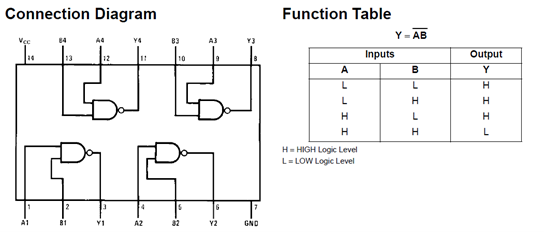
\includegraphics[width=0.8\textwidth]{pic/7400.png}
%            \caption{7400}
%     \label{}
%     \end{minipage}
%     \hspace{0.05\textwidth}
%     \begin{minipage}{0.3\textwidth}
%     \centering
%            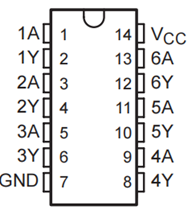
\includegraphics[width=0.8\textwidth]{pic/7404.png}
%            \caption{7404}
%     \label{}
%     \end{minipage}
% \end{figure}
\begin{figure}[H]
    \centering
    \begin{minipage}{0.3\textwidth}
    \centering
           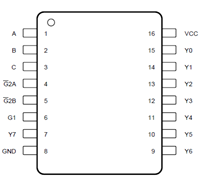
\includegraphics[width=0.8\textwidth]{pic/74138.png}
           \caption{74138}
    \label{}
    \end{minipage}
    \hspace{0.05\textwidth}
    \begin{minipage}{0.3\textwidth}
    \centering
           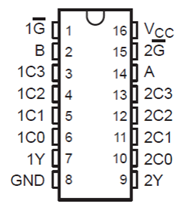
\includegraphics[width=0.8\textwidth]{pic/74153.png}
           \caption{74153}
    \label{}
    \end{minipage}
\end{figure}
\section{实验原理}
题目要求设计一个一位的算数逻辑运算单元ALU,要求实现4种功能。在这里不妨定义输入端为A、B和C,其中A为被加数或被减数,B为加数或减数,C为算数运算中低位向本位的进位;命令数码为$S_1,S_0$,设置三个输出端:F表示运算的本位,CO表示算数运算时的进位或借位,Z指示运算的类型。现在定义功能代码如下:
\begin{table}[H]
    \centering
    \caption{功能代码$S_1S_0$定义}
    \begin{tabular}{cccc}
    \hline 
        $S_1$ & $S_1$ & $Z$ & 运算类型\\ \hline 
        0 & 0 & 0 & 或\\
        0 & 1 & 0 & 与\\
        1 & 0 & 1 & 减\\
        1 & 1 & 1 & 加\\ \hline 
    \end{tabular}
    \label{tab:功能代码$S_1S_0$定义}
\end{table}
按所给的定义,给出真值表,其中Plus表示加法运算的本位,Minus表示减法运算的本位,And表示与运算的本位,Or表示或运算的本位,CO(Plus)表示加法运算的进位,CO(Minus)表示减法运算的借位。
\begin{longtable}{|p{1cm}<{\centering}| p{1cm}<{\centering} |p{1cm}<{\centering}| p{1cm}<{\centering} |p{1cm}<{\centering}|p{1cm}<{\centering}|p{1cm}<{\centering}|p{2cm}<{\centering}|p{2cm}<{\centering}|}%手动调间距
\caption{真值表}
\hline 
  A & B & C & Plus & Minus & And & Or & CO(Plus) & CO(Minus) \\ \hline
  0 & 0 & 0 & 0 & 0 & 0 & 0 & 0 & 0\\
\hline
  0 & 0 & 1 & 1 & 1 & 0 & 0 & 0 & 1 \\
\hline
  0 & 1 & 0 & 1 & 1 & 0 & 1 & 0 & 1 \\
\hline
  0 & 1 & 1 & 0 & 0 & 0 & 1 & 1 & 1 \\
\hline
  1 & 0 & 0 & 1 & 1 & 0 & 1 & 0 & 0 \\
\hline
  1 & 0 & 1 & 0 & 0 & 0 & 1 & 1 & 0 \\
\hline
  1 & 1 & 0 & 0 & 0 & 1 & 1 & 1 & 0 \\
\hline
  1 & 1 & 1 & 1 & 1 & 1 & 1 & 1 & 1 \\
\hline

\end{longtable}
容易看出,加法本位和减法本位的真值表一样,所以函数表示式也一样
\begin{equation}
    Plus=Minus=A\oplus B \oplus C
\end{equation}
而进位或借位的表达式不容易直接看出,但通过列卡诺图可以得到。对应真值表做出CO(Plus)和CO(Minus)的卡诺图
\begin{table}[H]
    \centering
    \caption{CO(Plus)卡诺图}
    \begin{tabular}{|c|c|c|}
\hline
\diagbox{AB}{C} & 0 & 1 \\
\hline
00 & 0 & 0 \\
\hline
01 & 0 & 1  \\
\hline
11 & 1 & 1  \\
\hline
10 & 0 & 1  \\
\hline
\end{tabular}
    \label{tab:CO(Plus)卡诺图}
\end{table}
\begin{table}[H]
    \centering
    \caption{CO(Minus)卡诺图}
    \begin{tabular}{|c|c|c|}
\hline
\diagbox{AB}{C} & 0 & 1 \\
\hline
00 & 0 & 1 \\
\hline
01 & 1 & 1  \\
\hline
11 & 0 & 1  \\
\hline
10 & 0 & 0  \\
\hline
\end{tabular}
    \label{tab:CO(Minus)卡诺图}
\end{table}
借助真值表可以化简得到两者的表达式:
\begin{equation}
    CO(Plus)=(A\oplus B)C+AB=AB+BC+AC=\sum m(3,5,6,7)
\end{equation}
\begin{equation}
    CO(Minus)=A'(B\oplus C)+BC=A'B+A'C+BC=\sum m(1,2,3,7)
\end{equation}
借助与或式,把输入端作为地址端,我们可以用最小项发生器74138来实现上述逻辑函数。

对于逻辑运算,出于减少器件类型的考虑,我们做如下变换
\begin{equation}
    A\cdot B=((AB)')'
\end{equation}
\begin{equation}
    A + B=(A'B')'
\end{equation}
这样就可以用7404和7400实现与运算和或运算了。

上述推导仅仅实现了四种逻辑/算数运算本身,并没有实现功能的选择。考虑到要同时选择运算类型和进位还是借位,这里我们采用双四选一数据选择器74153来实现.把$S_1S_0$作为选择端输入,对应于上文的功能编码规定,应该将或、与、减、加四种运算的结果分别送到第一片四选一数据选择器的第0,1,2,3个数据端。相对应地,把CO(Plus)和CO(Minus)送到第二片数据选择器的第3,2个数据端,而把第1,0个数据端接地。

注意到这样一个事实:当功能编码选择到算数运算时,进位端理应失效,但进位端本身的0或1只携带进位信息;换句话说,进位端本身并不能表示自己是不是有效输出,在逻辑运算时也会输出“进位”或“借位”。这显然不合理,需要额外一个数据端口的指示。为此我们选择构造输出端Z,当Z=1时,对应算数运算,此时的进位端有效;当Z=0时,表示进位端无效,此刻电路做逻辑运算。
\section{电路设计与实现}
\subsection{电路仿真图}
在Multisim中连接好电路仿真图
\begin{figure}[H]
    \centering
    \includegraphics[width=0.75\linewidth]{pic/Multisim仿真图.png}
    \caption{Multisim仿真图}
    \label{fig:enter-label}
\end{figure}
借助字发生器和逻辑分析仪,可以很方便地检验输出是否正确,下面是逻辑分析仪的截图。上半部分从上到下分别表示$F,CO,S_0,S_1$,中间部分从上到下表示$C,B,A$的输入波形。
\begin{figure}[H]
    \centering
    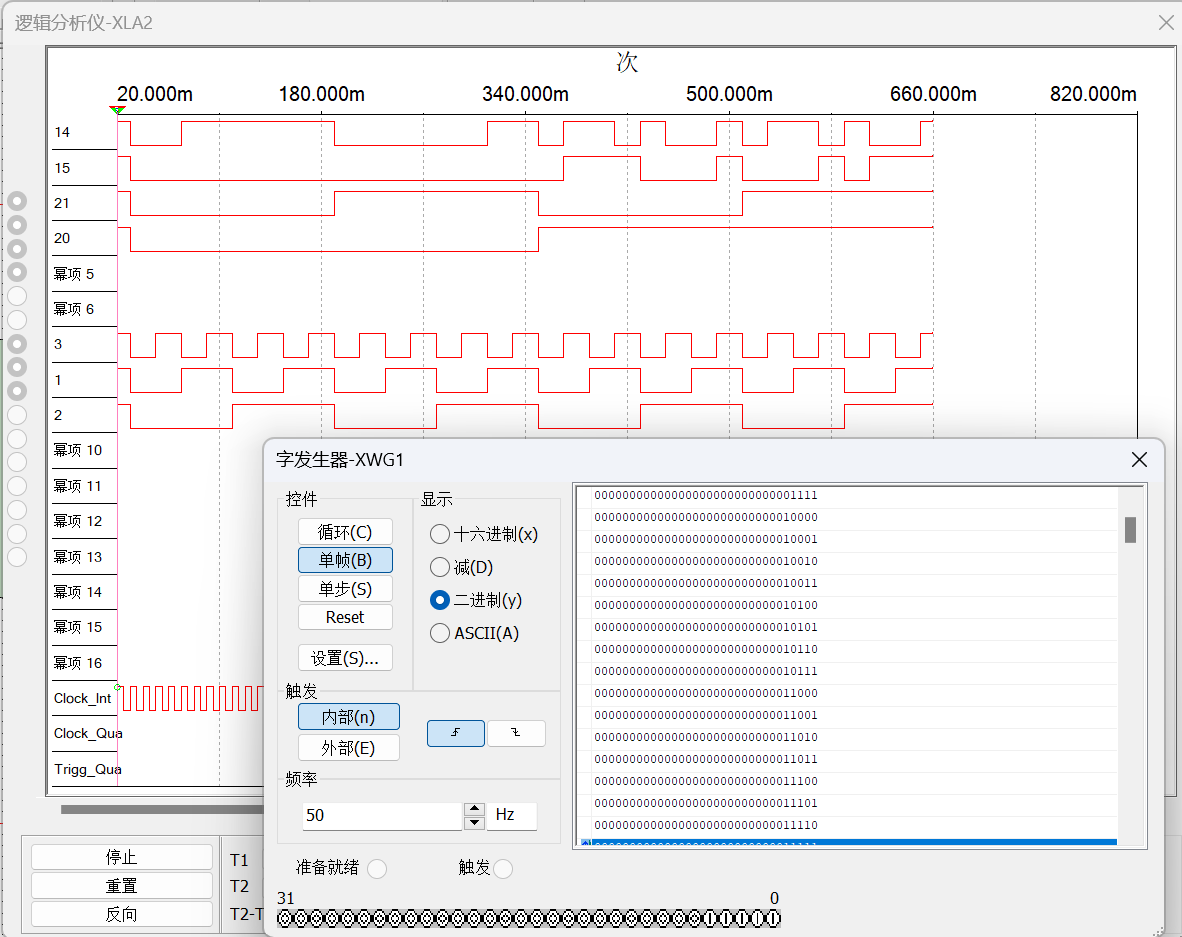
\includegraphics[width=0.75\linewidth]{pic/image.png}
    \caption{逻辑分析仪截图}
    \label{fig:enter-label}
\end{figure}
\subsection{电路实物图}
按电路仿真图搭好实物电路图
\section{功能测试}
\begin{figure}[H]
    \centering
    \includegraphics[width=0.5\linewidth]{pic/实物电路图.jpg}
    \caption{实物电路图}
    \label{fig:enter-label}
\end{figure}
%逐步测试及其调整
%pockelab、截图要一图一行才看得清楚
\begin{figure}[H]
    \centering
    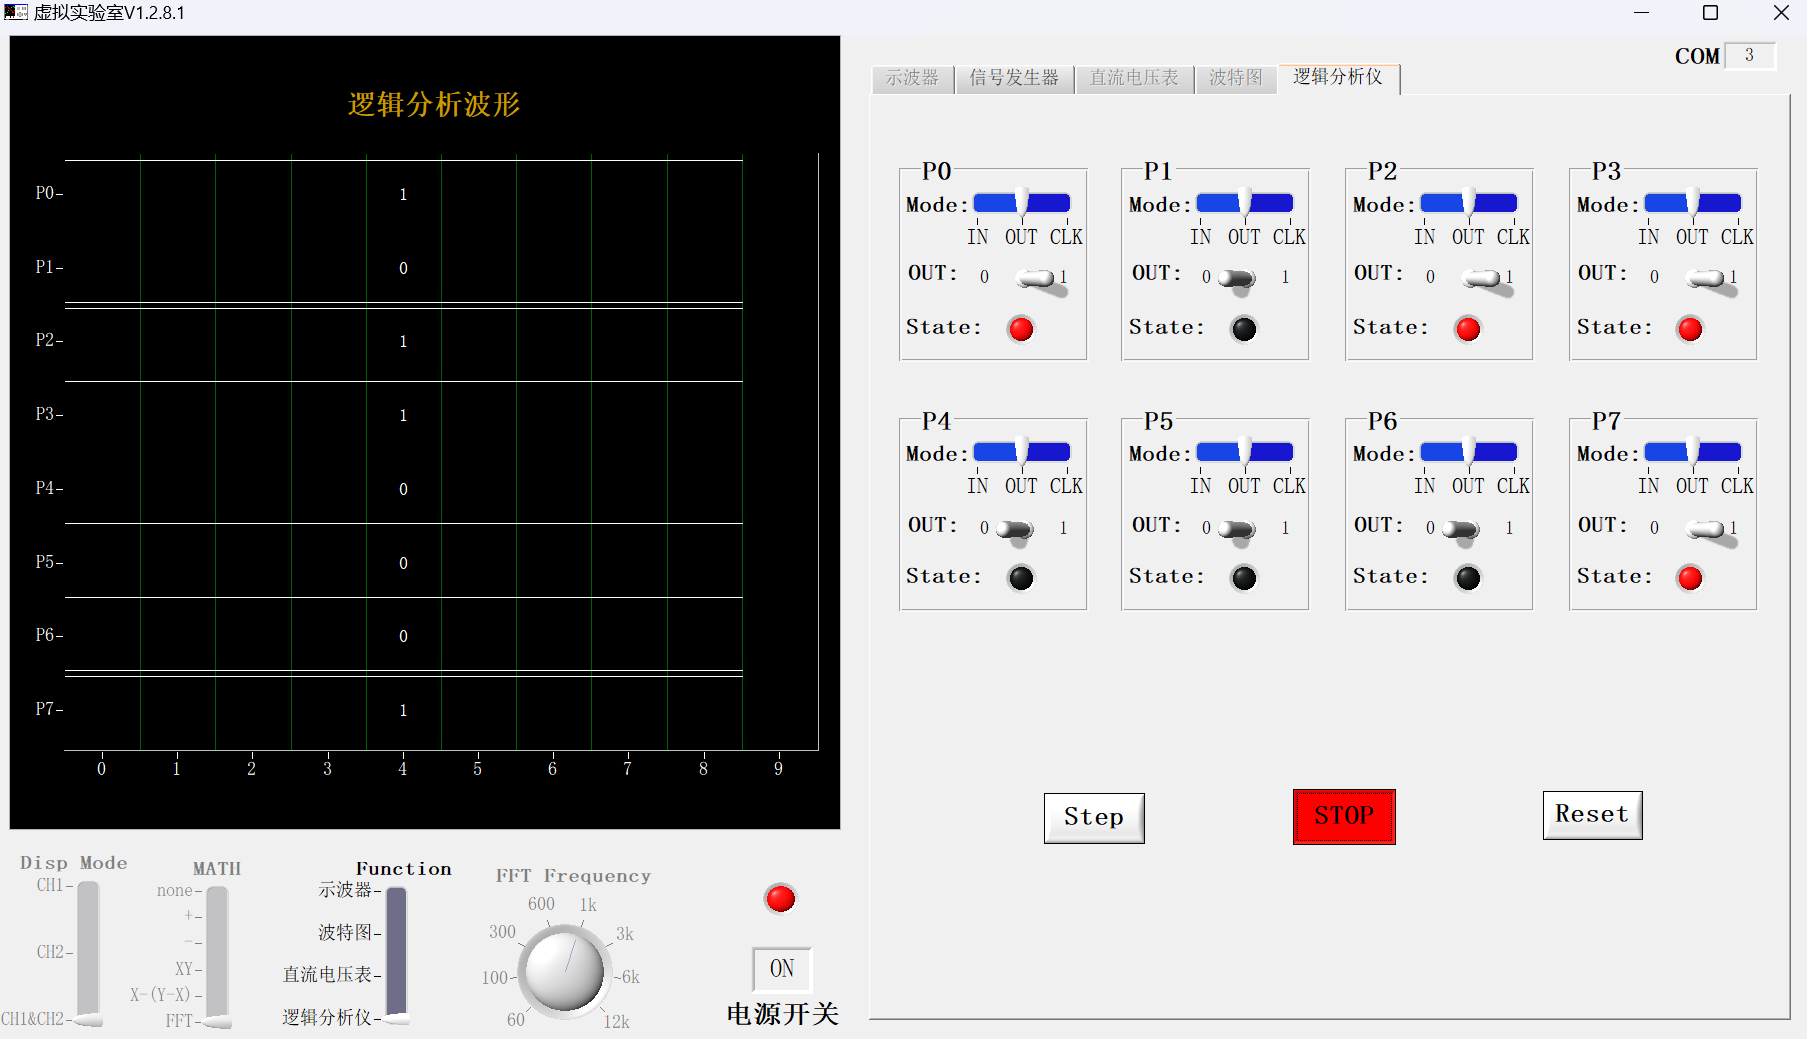
\includegraphics[width=0.5\linewidth]{pic/pocketlab.png}
    \caption{Pocketlab界面截图}
    \label{fig:enter-label}
\end{figure}
对实物电路进行检验。为了方便指示运算类型,将输出Z取反接到红色LED灯上,灯亮即警告进位无效,表示是逻辑运算。通过检测发现该电路功能正确且运行良好。
\section{实验总结与反思}
% 本次实验总体来说较为顺利,需求分析、逻辑表达、电路设计、仿真测试各个环节都没有遇到太大问题。但仍在以下几个方面有待提升
\begin{enumerate}
    \item 思考的周密性有待提升。本题做的是一位ALU,理应考虑与其他ALU级联的功能要求。但第一版电路设计没有考虑来自低位向本位的进位(Multisim仿真图如下),把这一版电路做完才考虑到有低位进位的可能,于是只能从头再来,极大地拖慢了进度。
    \item Multisim仿真经验增加。本实验涉及的输入端一共有5个,采用字发生器和逻辑分析仪可以简化仿真流程,但是在使用这两种虚拟仪器的时候发现一些问题:同样的输出,在逻辑分析仪上显示正常按既定功能工作,但是若用LED灯指示,结果与逻辑分析仪有出入。刚开始以为是电平不匹配造成的,但是测试发现,运行同样的测试字节,LED灯亮对应的最小项不一样,这排除了是电平的问题。后来通过仔细观察逻辑分析仪,发现了问题所在:因为要对最小项逐个检查,字发生器设置在单步模式,但逻辑分析仪和字发生器的节拍没有匹配好,导致字发生器当前的输入信号(这实时地反映到了LED上)与逻辑分析仪的显示波形有极其微小的错位,所以看起来不一样。有鉴于此,今后分析时宜选择逻辑分析仪进行功能检查,并要注意调好字发生器的频率。
\end{enumerate}
\begin{figure}[H]
    \centering
    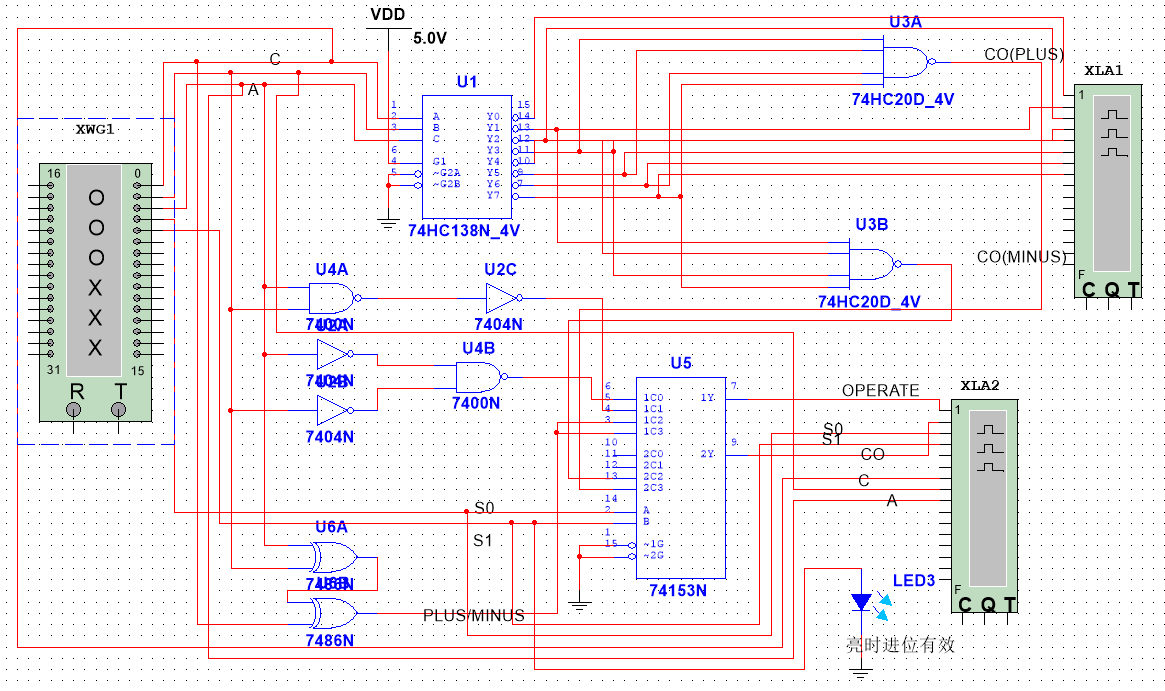
\includegraphics[width=0.5\linewidth]{pic/Multisim仿真图旧.png}
    \caption{第一版电路设计}
    \label{fig:enter-label}
\end{figure}
\end{document}